\chapter{Eulerian Domain: Finite Element Method}
\label{ch:eulerian}
	\lsymb[f]{$\mathcal{T}_h$}{Finite Element mesh}{-}{th}		
	\lsymb[f]{$T$}{Cell of Finite Element mesh}{-}{t}			
	
	\lsymb[f]{$v$}{Test function}{-}{v}				
	\lsymb[f]{$V$}{Trial vector function space}{-}{vte}				
	\lsymb[f]{$\hat{V}$}{Test vector function space}{-}{vtr}					
	\gsymb[f]{$\Omega$}{Fluid domain}{-}{x}	
	\gsymb[f]{$\Omega_E$}{Eulerian fluid domain}{-}{xe}	
	\gsymb[f]{$\Omega_L$}{Lagrangian fluid domain}{-}{xl}	
	\gsymb[f]{$\partial \Omega$}{Boundary of the domain $\Omega$}{-}{xdd}	

%------------------------------------------------------------------------------------------------------
%------------------------------------------------------------------------------------------------------
%------------------------------------------------------------------------------------------------------
%\section{Purpose of eulerian domain}
Standard \printAcron{Computation Fluid Dynamics}{CFD} method discretizes the fluid into smaller regions, known as grids, and solves the set of Navier-Stokes equations in this region. This type of formulation is referred to as an Eulerian method, as we are evaluating the change of flow property in a given volume.

For the hybrid method, we use the Navier-Stokes grid formulation in the near-body region. The advantage of using the Eulerian method at this region is that it is much more efficient in resolving the boundary layer than the Vortex Particle Method. We can directly enforce the wall boundary condition at the wall boundary of the Eulerian domain, solving the problem of vorticity generation of the body. In the hybrid coupling strategy, we can then interpolate this newly resolved near-wall solution on to the Lagrangian domain, where the vortex blobs can efficiently evolve the particles.

The various approaches to solve the fluid dynamics problem from a Eulerian reference frame. \indexAcron{Finite Volume Method }{FVM}, \indexAcron{Finite Difference Method}{FDM}, and \indexAcron{Finite Element Method}{FEM} are the common choice for solving the Navier-Stokes problem and differ by the way they approach to solve the problem. FVM divides the domain into volumes where it enforces the conservation of mass and momentum in each sub-domains. FDM divides the domain into nodes and use local Taylor expansions to approximate the partial differential equations. FEM divides the domain into elements and solves the problem using variational calculus. So in the end, the choice of Eulerian method does not have a direct impact on the coupling with the Lagrangian method as the purpose of the Eulerian method is only to efficiently, and accurately resolve the near-body region of the body.

We have decided to use the FEM packages provided by the \fenics project as they have be already implemented efficient, multi-threaded algorithms for solving the partial differential equation. Furthermore, they provide extensive features for future developments such as adaptive mesh refinement, fluid-structure interaction, and efficient computation of turbulent flow.

\section{Introduction to Finite Element Method}

\printAcron{Finite Element Method}{FEM} is numerical method to solve for the solution of a given partial differential equation. It is solved by describing it as a variation problem, giving us an approximate solution for the boundary value problem \cite{Brenner2002}. So the FEM approximates the unknown variables and converts the partial differential equations to a set of algebraic equations, which makes them easier to solve. It was traditionally used for solid mechanics (e.g for the analysis of aircraft structures \cite{RAO2011}), but have since then used to solve fluid dynamics problems \cite{Guermond2006a} \cite{Johnston2004a} \cite{Guermond2003a}.

\subsection*{Finite element discretization}

Finite Element method solves problem by dividing the domain of interest into smaller, simpler regions known as ``elements". These ``elements" are connected at the joints which are called nodes or nodal points. We use these sets of node and elements to represent the actual variation in the field (such as the displacement, the velocity, the pressure or the temperature) using simple functions, known as the basis functions. Thus, we have transformed the domain of interest into finite number of \indexAcron{Degrees of Freedom}{DOF}. We combine the set of equations of the element into a global system of equations to solve for the unknown.

	\begin{figure}[b]
	\centering
	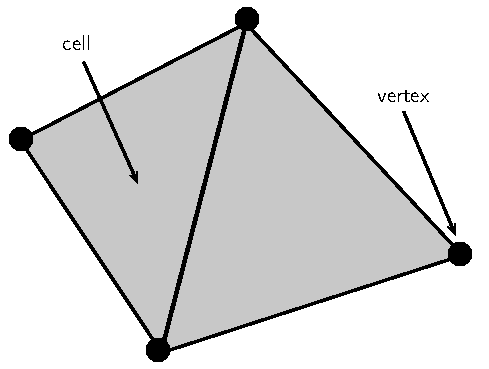
\includegraphics[width=0.4\linewidth]{./figures/eulerian/finiteElementDefinitions.pdf}
	\caption{A two-dimensional Finite Element geometry. The cell represents the area of the element, and vertices are the edges of the cell.}
	\label{fig:finiteElementDefinitions}
	\end{figure}

A FE discretization in 2-D can be seen in figure \ref{fig:finiteElementDefinitions}. The figures shows two connected elements, where the cells represent the area of the element, and the vertices of the cell represents the nodes of the element. The finite number of cells $\mathcal{T}_h = \{T\}$ of the fluid domain $\Omega$, together makes the mesh of the Eulerian domain. As shown in figure \ref{fig:finiteElementDefinitions}, the cells of the finite element in 2-D, are made of simple geometrical shapes such as triangles or quadrilaterals. There are two approaches to discretize the domain: structured or unstructured mesh. The structured mesh has cells oriented in a structured pattern, and is the simplest approach in discretizing the mesh. The advantage of such a discretization is that it is possible to make a simple data structure which can be used to perform efficient computation. The downside to such discretization is that the mesh quality deteriorates as one increases the complexity of the domain. However, the FEM enables us to perform an unstructured discretization of the domain, as shown in figure \ref{fig:cylinderFiniteElementDiscretization}. The figure shows the unstructured discretization of the fluid domain around the cylinder $\Omega_E$, connecting the rectangular outer boundary of the fluid to the circular no-slip boundary of the body in a simple fashion. This shows that even though the unstructured method formulation is more complicated that the structured formulation, we have the advantage that the mesh quality does not deteriorate as the domain becomes more complex.

There are several algorithms for mesh generation. The standard approach is to employ the Delaunay triangulation method derived from the Voronoi diagram concept \cite{Carey1997}. This divides the domain into a set of triangles, as shown in figure \ref{fig:cylinderFiniteElementDiscretization}. This type of mesh generation allows us to connect different shapes of boundary with each other. Furthermore, this triangulation method be controlled by predefining the boundary element nodes using a transfinite interpolation.

\begin{figure}[t]
        \centering
        \begin{subfigure}[b]{0.5\textwidth}
                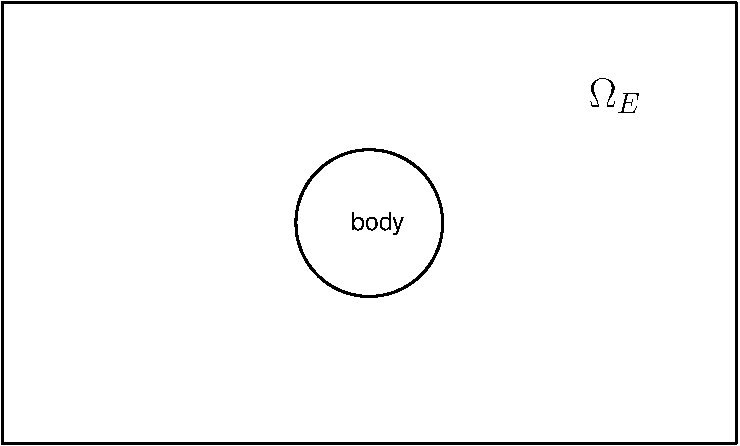
\includegraphics[width=\textwidth]{figures/eulerian/cylinderPreDelauney-crop.pdf}
                \caption{Fluid domain $\Omega_E$ around the cylinder}
                \label{fig:cylinderPreDelauney}
        \end{subfigure}%
        ~ %add desired spacing between images, e. g. ~, \quad, \qquad etc.
          %(or a blank line to force the subfigure onto a new line)
        \begin{subfigure}[b]{0.5\textwidth}
                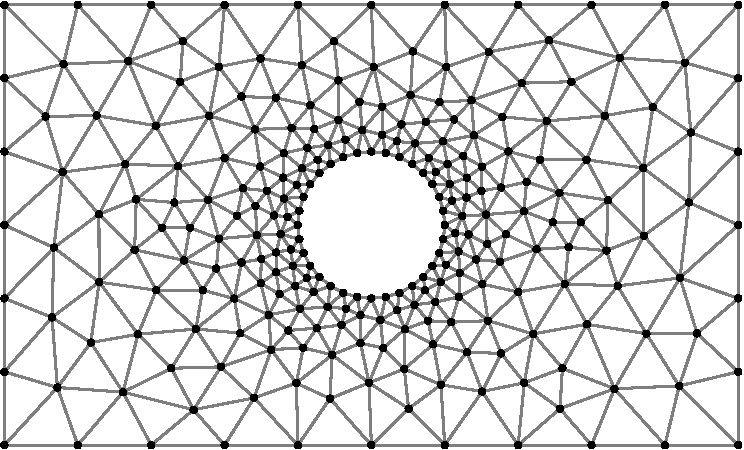
\includegraphics[width=\textwidth]{figures/eulerian/cylinderDelauney-crop.pdf}
                \caption{Delaunay triangulation of the fluid}
                \label{fig:cylinderDelauney}
        \end{subfigure}
        \caption{Delaunay triangulation of the fluid around a cylinder resulting in unstructured mesh with controllable cell sizes.}
        \label{fig:cylinderFiniteElementDiscretization}
\end{figure}	

\subsection*{Finite element function and function space}

The finite element is defined using a triple ($T, \mathcal{V}, \mathcal{L}$), as defined Ciarlet \cite{Ciarlet1972b} and used by \fenics Project \cite{Logg2012b}, where the domain $\Omega$ is divided into cell $T$, the space $\mathcal{V} = \mathcal{V}(T)$ is a finite dimensional function space on $T$ of dimension $n$, and $\mathcal{L} = \left\{ \ell_1,\ell_2,...,\ell_n \right\}$ is the set of degrees of freedom for the basis.

When the domain $\Omega$ is divided into cells $T$, we can define the function and the function space of the Finite element problem. For each cell, a local function space $\mathcal{V}$ can be defined to collectively construct the global function space $V$. Any given function $u \in V$ is a expressed in a linear combination of basis functions $\{\phi_1,\phi_2,...,\phi_N\}$  of the function space $V$, 
	\begin{equation}
	u(x) = \sum_{j=1}^N U_j\phi_j(x).
	\end{equation}

There are several types of Finite Element families: the Brezzi-Douglas-Marini, the Crouzeiz-Raviart, the Discontinuous Lagrange, the Hermite, and the Lagrange elements \cite{Logg2012b}. Each has its own advantage such as the Discontinous Lagrange, or \indexAcron{Discontinous Galerkin}{DG} element consists of discontinuous functions. It was originally introduced for hyperbolic problem by Reed and Hill in 1973 \cite{Reed1973a}. The method is able to conserve mass at each element, has a high-order accuracy, and is robust in solving the advection problem. However for the current problem, we will rely on the standard Lagrange elements, known as the \indexAcron{Continuous Galerkin}{CG}, which are based on the Lagrange polynomials \cite{Chen2011}. 

The Lagrange elements are most used and is the simpler types of finite element. They belong to the space $H^1$, which a Sobolev space containing functions $u$ such that $u^2$ and $\left|\nabla u\right|^2$ have finite integral in the domain $\Omega$ \cite{Logg2012b}. The Lagrange element uses point evaluation for the degrees of the freedom, where a DOF in $(x,y)$ denotes the point evaluation of the function $u$, $\ell(u) = u(x,y)$. We can have a Lagrange elements of various orders $q = 1, 2,...$, where $q$ is the degree of the Lagrange polynomial $\mathcal{P}_q$ on the domain at$T$. For the 2-D case, the cells of the finite element are triangles, and the dimension $n$ of the finite element is determined by,
	\begin{equation}
	n(q) = \frac{1}{2}(q + 1)(q + 2).
	\end{equation}

For $q=1$, we have a simple Lagrange triangle $\mathrm{CG}_1$, known as the Courant triange \cite{Courant1943}, with $3$ DOFs. For a higher order finite element, we can set $q=2$, giving us a Lagrange element $\mathrm{CG}_2$ with $6$ DOFs per cell. Figure \ref{fig:continuousGalerkin} shows the two Lagrange triangles $\mathrm{CG}_1$ and $\mathrm{CG}_2$ for $q = 1$ and $q=2$ respectively. The Courant triangle has the DOFs located at the vertices of the cell, and the higher order $CG_2$ has $3$ additional DOFs, all located midway between the vertices.

	\begin{figure}[t]
	\centering
	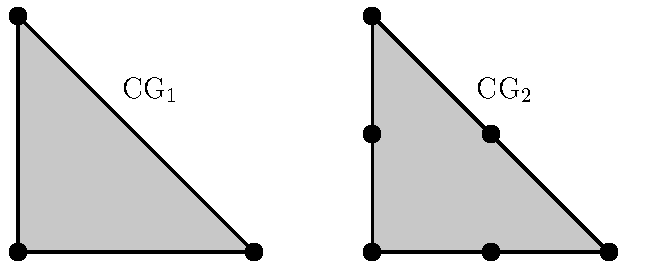
\includegraphics[width=0.6\linewidth]{./figures/eulerian/continuousGalerkin.pdf}
	\caption{The Lagrange $\mathrm{CG}_q$ triangle for $q = 1, 2$. The triangles have $3$ and $6$ DOFs respectively ({\color{black}{$\bullet$}}, black dot).}
	\label{fig:continuousGalerkin}
	\end{figure}



\subsection*{Variational formulation}
\label{subsec:variationalProblem}

To solve a basic problem such as a Poisson equation numerically, we need to convert it into a variational problem. The methodology is followed from the \fenics tutorial provide by Langtangen \cite{Logg2012b}. A 1D Poisson problem is given as,
	\begin{equation}
	\begin{aligned}
	- \nabla^2 u(x) &= f(x), \qquad x\ \mathrm{in}\ \Omega,\\
	u(x) &= u_0(x), \qquad x\ \mathrm{on}\ \partial\Omega.
	\end{aligned}
	\label{eq:poissonEq}
	\end{equation}
	
We can transform equation \ref{eq:poissonEq} into a variational form by multiplying it with a test function $v$, and integrating it over the domain $\Omega$,
	\begin{equation}
	- \int_{\Omega} \left(\nabla^2 u\right)v\ \mathrm{d}x= \int_{\Omega} fv\ \mathrm{d}x, \qquad \forall\ v \in \hat{V}.
	\label{eq:poissonEqVariationFormA}
	\end{equation}

In variational form equation \ref{eq:poissonEqVariationFormA}, the function $u$ is known as the trial function, and is what we are trying to approximate. The trail function $u$ lies in the trail function space $V$, and the test function $v$ lies in the test function space $\hat{V}$. When performing integration by parts, the test function $v$ is required to be zero at regions where $u$ is known. So, the additional terms cancel and we get,

	\begin{equation}
	- \int_{\Omega} \nabla u \nabla v\ \mathrm{d}x= \int_{\Omega} fv\ \mathrm{d}x \qquad \forall\ v \in \hat{V}
	\label{eq:poissonEqVariationFormB}
	\end{equation}

This form is referred to as the ``weak-form" of the original Poisson equation and is valid for all $v$ in the trial space $\hat{V}$. The inner product of two function $f$ and $g$ is defined as,
	\begin{equation}
	\langle f,g \rangle = \int_{\Omega}fg\ \mathrm{d}x,
	\end{equation}
so equation \ref{eq:poissonEqVariationFormB} can be summarized as,
	\begin{equation}
	\langle \nabla u,\nabla v \rangle = \langle f,v \rangle, \qquad \forall\ v \in \hat{V}.
	\end{equation}

In order to solve this continuous problem numerically, we must transform it into discrete variational problem,

	\begin{equation}
	- \int_{\Omega} \nabla u_h \nabla v\ \mathrm{d}x= \int_{\Omega} fv\ \mathrm{d}x \qquad \forall\ v \in \hat{V}_h \subset \hat{V},
	\label{eq:poissonEqDiscreteVariational}
	\end{equation}

where $u_h$ is the discrete function in the discrete space $V_h$ which is a subset of $V$, and the discrete function space $\hat{V}_h$ is a subset of $\hat{V}$. A common choice for the function space is linear triangular element with three nodes, as shown in figure \ref{fig:continuousGalerkin}, where $\hat{V}_h$ and $V_h$ are described by piecewise linear functions of the triangle. At the boundary, the functions in the test space is zero, whereas the functions in the trail space is equal the boundary condition $u_0$.  The equation \ref{eq:poissonEqDiscreteVariational} can be transformed into,
	\begin{equation}
	a\left(u,v\right) = L(v),
	\label{eq:weakForm}
	\end{equation}
where,
	\begin{equation}
	a\left(u,v\right) = - \int_{\Omega} \nabla u \nabla v\ \mathrm{d}x,
	\end{equation}
and
	\begin{equation}
	L(v)=\int_{\Omega}fv\ \mathrm{d}x.
	\end{equation}

The variable $a(u,v)$ and $L(v)$ is the denoted as the bilinear and linear form, respectively. For simplicity, we will ignore the discrete notation (i.e $\{\cdot\}_h \rightarrow \{\cdot\}$). To solve for the discrete solution we substitute,	
	\begin{equation}
	u = \sum_{j=1}^{N} U_j \phi_j,
	\label{eq:trialDiscrete}
	\end{equation}
the linear combination of the basis function $\phi_j$, spanning the function space $V$, into $a\left(u,v\right)$. The test function is linear combination of the basis function $\hat{\phi}_i$, spanning the test space $\hat{V}$, which is defined as
	\begin{equation}
	v=\sum_{i=1}^{N} \hat{\phi}_i.
	\label{eq:testDiscrete}
	\end{equation}
	
The test function $v$ is taken to be zero at the boundary and one everywhere else. Substituting equation \ref{eq:trialDiscrete} and \ref{eq:testDiscrete} into equation \ref{eq:weakForm} gives,
	
	\begin{equation}
	\sum_{j=1}^N a(\phi,\hat{\phi}_i)\ U_j = L(\hat{\phi}_i).
	\end{equation}

Thus, we have to solve a linear system of equations given as,

	\begin{equation}
	\mathbf{A}U = b,
	\label{eq:linearSysOfEq}
	\end{equation}	
	
where $\mathbf{A}_{ij} = a(\phi_j,\hat{\phi}_i)$ is the coefficient matrix, and $b$ is the \printAcron{Right-Hand Side}{RHS} containing the knowns of the problem.
 	
%------------------------------------------------------------------------------------------------------
%------------------------------------------------------------------------------------------------------
%------------------------------------------------------------------------------------------------------
\section{Solving the Finite Element problem}

To solve this linear system of equations, equation \ref{eq:linearSysOfEq}, we use the \fenics Project that has implemented a comprehensive library of finite elements, and high performance linear algebra. The \dolfin library from the \fenics Project was used to define the Eulerian domain of the hybrid coupling scheme.

In order to generate the mesh of the fluid domain, we used \gmsh, a three-dimensional finite element mesh generator which proves a fast, light and user-friendly meshing tools.

\subsection{Introduction to FEniCS Project}

	\begin{figure}[t]
	\centering
	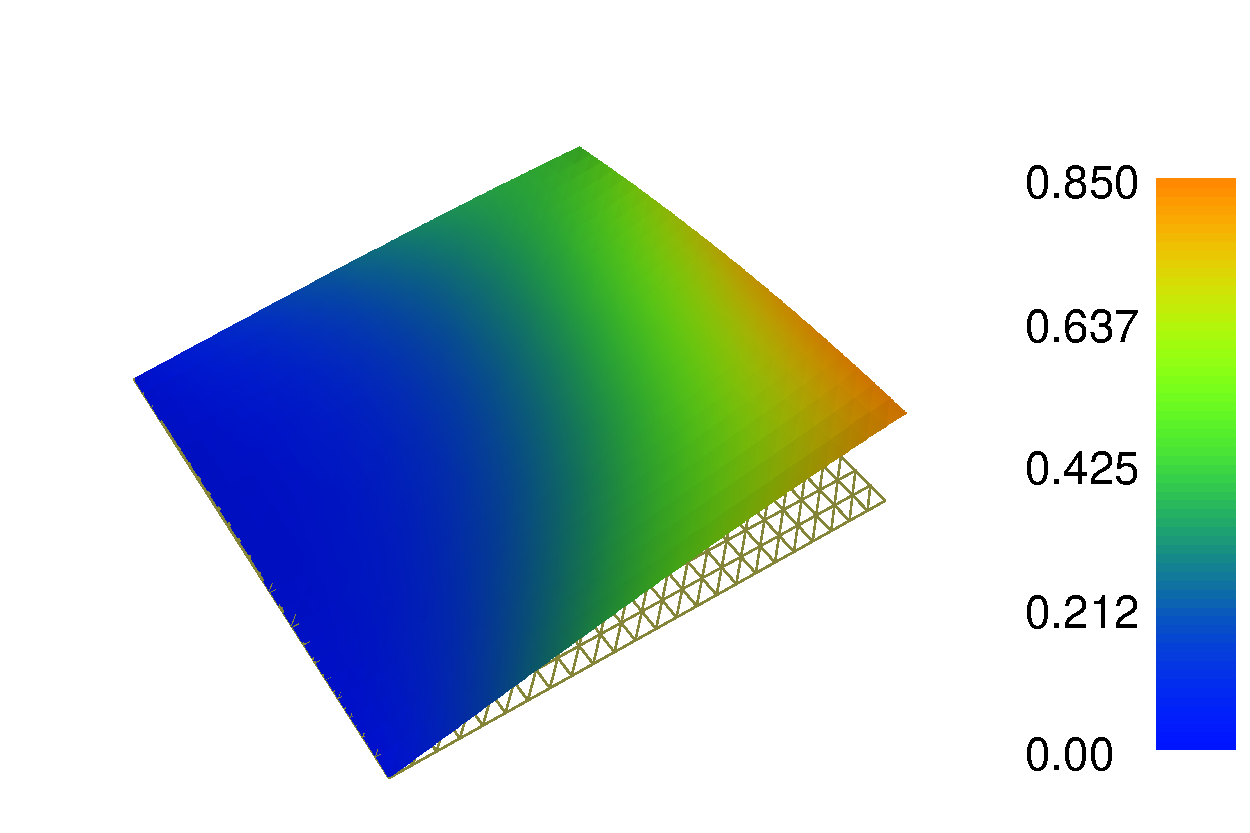
\includegraphics[width=0.5\linewidth]{./figures/eulerian/dolfinExampleFigure-rotated270.pdf}
	\caption{\dolfin VTK plot of the Poisson solution, given by the problem, source code listing \ref{lst:pycode-poisson}.}
	\label{fig:dolfinExampleFigure}
	\end{figure}

The \fenics Project is a collaborative work of various universities, that developed tools to automated Finite Element Methods for solving the solutions of differential equation \cite{FenicsAbout}. It was a project originated in 2003 with the research collaboration of University of Chicago and Chalmers University of Technology with Logg,  Mardal, and Wells \cite{Logg2012b}. Since then, it has been expanded to various institutes such as Royal Institute of Technology, Simula Research Laboratory, Univeristy of Cambridge, and Delft Universty of Technology.

	\begin{listing}[p]
	\inputminted[fontseries=courier,obeytabs,fontsize=\footnotesize,mathescape,linenos,numbersep=5pt,frame=lines,framesep=2mm,xleftmargin=20mm,xrightmargin=20mm]{python}{figures/eulerian/dolfinExample.py}
	\caption{A complete program for solving the Poisson problem and plotting the solution. The Poisson problem is given as $-\nabla^2{u} = f$, where $u_0 = \sin{x}\cdot\cos{y}$ on the boundary and $f=2$. The code is written in \python using \dolfin 1.2 library}
	\label{lst:pycode-poisson}
	\end{listing}

The consists of various libraries such as UFC, UFL, FIAT, INSTANT and mainly \textsc{Dolfin}. \dolfin is the core library aimed at automating the solution of partial differential equations using finite element method \cite{Logg2011}. It uses automated code generation maintaining high level of mathematical expressions and internally providing efficient, multi-threaded performance using the \indexAcron{Message Passing Interface}{MPI}. It used built-in linear algebra backend such as PETSc, TRILINOS/EPECTRA, uBLAS, and MTL4.

The Poisson problem to with the source code was evaluated is given by,

	\begin{equation}
	-\nabla^2 u = f,
	\end{equation}

where $f=2$ and $u(x) = u_0(x) = \sin x \cdot \cos y$ on boundary $\partial \Omega$ can be automated using the \texttt{DOFLIN} library. The solution algorithm follows from section \ref{subsec:variationalProblem}. The ection \ref{subsec:variationalProblem} can be seen in listing \ref{lst:pycode-poisson}.

\subsection{Mesh generation using GMSH}

The proper generation of the fluid mesh is an important aspect of the Finite Element method. It is a non-trivial process, as a non-ideal mesh can be computationally expensive, given un-precise data, and even cause convergence issues. There have been literatures dedicated just to improve the mesh generation, that focuses of improving the quality of the mesh thereby increasing the quality of the data and increasing the robustness of the simulation \cite{Hansen2005}. 

We used \gmsh an open-source finite element mesh generator, which has implemented a user-friendly interface and fast algorithms, developed by Geuzaine and Remacle \cite{Geuzaine2009a}. Its kernel uses \textsc{BLAS} and LAPACK linear algebra packages, and is written in C++. It allows for scriptability making it ideal to chain it with our current \python code project for automation.

\section{Solving Incompressible Navier-Stokes Equations}
The finite element method will be used to describe the Eulerian domain of the hybrid scheme. In the Lagrangian domain, we have used the vorticity-velocity formulation of the Navier-Stokes to describe the evolution of the vorticity in the wake. In the Eulerian domain, where have the no-slip boundary, we have decided to use the primitive variables for formulation the fluid dynamics problem. 

\subsection{Velocity-pressure formulation}
The velocity-pressure formulation is the standard formulation of the Navier-Stokes equations of the fluid dynamics problem. The 2-D incompressible Navier-Stokes equations of unit fluid density is given as,

	\begin{subequations}
	\begin{align}
	\frac{\partial \mathbf{u}}{\partial t} + \mathbf{u}\cdot\nabla\mathbf{u} - \nabla \cdot \sigma &= f,\\
	\nabla \cdot \mathbf{u} = 0,
	\end{align}	
	\label{eq:2Dns}
	\end{subequations}

where $\sigma$ is the Cauchy stress tensor given as,

	\begin{equation}
	\sigma(\mathbf{u},p) = 2\nu\epsilon(\mathbf{u}) - p\mathbf{I}.
	\end{equation}

The problem contains our two unknowns which are the velocity field $\mathbf{u}$ and our pressure field $p$. The problem is function of the viscosity $\nu$, external force $f$ and the symmetric gradient,

	\begin{equation}
	\epsilon(u) = \frac{1}{2} \left(\nabla \mathbf{u} + \nabla \mathbf{u}^{\mathrm{T}}\right).
	\label{eq:symGrad}
	\end{equation}

The velocity field $\mathbf{u}$ is vector function that lies on the vector-valued function space $V$ and scalar pressure field $p$ lies on the function space $Q$.

\subsection{Incremental pressure correction scheme}

The algorithm to solve the Navier-Stokes problem was first demonstrated by Chorin in 1968 \cite{Chorin1968}, nowadays referred to as Chorin's projection method or non-incremental pressure correction scheme. The process relied on first computing a tentative velocity by initially neglecting the pressure in the momentum equation of the Navier-Stokes problem, equation \ref{eq:2Dns}. The velocity field is corrected by determining the pressure field satisfying a divergence free vector field. This method however does not satisfy the discrete incompressibility constraint exactly and so Goda, has introduced a improvement to scheme known as the \indexAcron{Incremental Pressure Correction Scheme}{IPCS}, Goda 1979 \cite{Goda1979a}.

The method computed the viscous term at the incremented time $(t_{n-1} + t_n)/2$ and used the stress formulation determining the corrected pressure \cite{Logg2012b}. The algorithms to the IPCS scheme can be summarized as follows:

	\begin{enumerate}
	\item \textbf{Compute the tentative velocity:} The tentative velocity given as $\mathbf{u}^{\star}$ is determined by solving
	
		\begin{equation}
		\begin{split}
		\langle D_t^n \mathbf{u}^{\star}, v \rangle &+ \langle \mathbf{u}^{n-1}\cdot\nabla\mathbf{u}^{n-1},v\rangle + \langle \sigma(\mathbf{u}^{n-\frac{1}{2}},p^{n-1}), \epsilon(v) \rangle \quad \\ &\quad+ \langle p^{n-1}\hat{\mathbf{n}},v\rangle_{\partial \Omega} - \langle v\hat{\mathbf{n}} \cdot (\nabla u^{n-\frac{1}{2}} )^{\mathrm{T}},v \rangle_{\partial \Omega} = \langle f^n,v \rangle,
		\end{split}
		\end{equation}
		
	where $\langle u,v \rangle = \int_{\Omega} u(x)v(x)\ \mathrm{d}x$ is the inner product of the two functions. The term $u^{n-\frac{1}{2}}$ is defined as $u^{n-\frac{1}{2}} = (u^{\star}+u^{n-1})/2$. The equation is given for all test function $v \in V$, with the valid dirichlet velocity boundary conditions at boundary $\partial \Omega$.
	
	\item \textbf{Determine the corrected pressure:} The corrected pressure $p^n$ is determined by solving
	
		\begin{equation}
		\langle \nabla p^n, \nabla q \rangle = \langle \nabla p^{n-1}, \nabla q\rangle - \langle \nabla \cdot u^{\star}, q \rangle / \Delta t_n
		\end{equation}
	
	with the valid pressure boundary condition, and the test function $q \in Q$. Using the corrected pressure, we can determine the final corrected velocity field. 
		
	\item \textbf{Determine the corrected velocity:} The corrected velocity field $u^n$ is determined by solving
	
		\begin{equation}
		\langle u^n, v\rangle = \langle u^{\star},v \rangle - \Delta t_n \langle \nabla(p^n - p^{n-1}),v \rangle,
		\end{equation}
		
	for the velocity boundary condition.
		
	\end{enumerate}
	
	\begin{figure}[t]
	\centering
	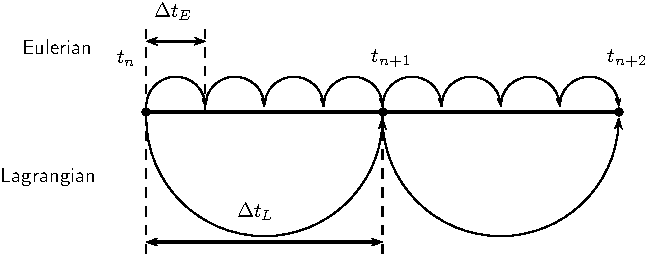
\includegraphics[width=0.7\linewidth]{./figures/eulerian/multiStep-crop.pdf}
	\caption{Eulerian multi-stepping to match the lagrangian $\Delta t_L$. The figures shows $\Delta t_L = 4 \Delta t_E$ and required $k_E = 4$ iterations to time march from $t_n$ to $t_{n+1}$.}
	\label{fig:multiStep}
	\end{figure}
	
	
This algorithm was implemented using \textsc{Dolfin}'s Krylov \textsc{Gmres} solver with absolute and relative error tolerance of \num{e-25} and \num{e-12} respectively. The program structure was based on the collection of benchmark and solvers provided by the \fenics examples scripts \cite{nsbench}.

The algorithm described above an explicit time marching scheme, also referred to as \indexAcron{Forward Euler}{FE}, which is the simplest time marching scheme. Therefore, for the time marching scheme to be stable, we require the CFL number satisfy the following condition:

	\begin{equation}
	\mathrm{CFL} = \Delta t_{\mathrm{max}} \frac{\lVert\mathbf{u}\rVert_{\mathrm{max}}(\nu +  \Delta h_{\mathrm{min}}\lVert\mathbf{u}\rVert_{\mathrm{max}})}{\Delta h_{\mathrm{min}}^2} \le 1.
	\end{equation}
	
This gives us the direct constraint on the maximum Eulerian time step size $\Delta t_{E,\mathrm{max}}$ which is function of the $\mathrm{CFL}$ number, maximum fluid velocity in the Eulerian domain $\lVert \mathbf{u} \rVert_{\mathrm{max}}$, the fluid viscosity $nu$ and the minimum mesh cell size $\Delta h_{min}$. When coupling with the Lagrangian method, we will see that $\Delta t_E \le \Delta t_L$ (Lagrangian time step size is ideally larger than Eulerian time step size), meaning that we will have to perform $k_E$ Eulerian sub-steps to reach the Lagrangian step, figure \ref{fig:multiStep}.

\subsection{Determining the vorticity field}

	\begin{listing}[t]
	\inputminted[fontseries=courier,obeytabs,fontsize=\footnotesize,mathescape,linenos,numbersep=5pt,frame=lines,framesep=2mm,xleftmargin=20mm,xrightmargin=20mm]{python}{figures/eulerian/vorticity.py}
	\caption{The \textsc{python} implementation of the vorticity calculation}
	\label{lst:pycode-vorticity}
	\end{listing}

The coupling between the Eulerian to Lagrangian method is through the transfer of the vorticity field $\omega$ from the Eulerian domain to the Lagrangian vortex blobs. The vorticity field $\omega$, is defined as,

	\begin{equation}
	\omega = \nabla \times u,
	\label{eq:vorticityEq}
	\end{equation}

and is defined as the curl of the velocity field $\mathbf{u}$. Using the IPCS scheme, the finite element method that we have employed solves for the velocity field and the pressure field. Therefore, to derive the vorticity field, we simply have to take the curl of our solution. However, as this evaluation have to be done at every step (i.e $t_n, t_{n+1}, ...$ of figure \ref{fig:multiStep}), we have to solve this problem in a efficient manner. An efficient process, that \textsc{FEniCS} has implemented, is by pre-assemble the known of the problem, so that the only terms we have to redefine the unknowns of the problem. To do this, we must first define equation \ref{eq:vorticityEq} in the variational (integral) form, 

	\begin{equation}
	\int_{\Omega} \omega \cdot v\ \mathrm{d}x = \int_{\Omega} (\nabla \times u) \cdot v\ \mathrm{d}x,
	\end{equation}

where $\omega = \sum_{j=1}^N \hat{\omega}_j\psi_j$, is a linear combination of basis function $\psi_j$, spanning the function space $W$. The variational form is summarized as

	\begin{equation}
	a(\omega,v) = L(v)
	\end{equation}

where $a(\omega,v)$ contains the knowns of the problem and can be pre-calculated to optimize the problem. $L(v)$ is the unknown of the problem which has to be recalculated every time we need to solve the problem. The \textsc{python} implementation of the algorithm is show in listing \ref{lst:pycode-vorticity} and we see the $\mathrm{LHS}$ of the problem is pre-evaluated using the \texttt{assemble} function of the \textsc{dolfin} library.

\subsection{Determining the body forces}

	\begin{listing}[t]
	\inputminted[fontseries=courier,obeytabs,fontsize=\footnotesize,mathescape,linenos,numbersep=5pt,frame=lines,framesep=2mm,xleftmargin=20mm,xrightmargin=20mm]{python}{figures/eulerian/forces.py}
	\caption{The \textsc{python} implementation of the force calculation}
	\label{lst:pycode-forceCalculation}
	\end{listing}

Once we solved for flow fields, it is a common strategy to verify the results using some sort of quantities. In aerodynamics, (especially in aerospace field), we like the evaluated the lift and drag coefficient of a given geometry and compare the results to available literature. In order to determine these coefficient, we must first determines the 
friction force and the pressure force acting on the no-slip boundary, or simply put, it is the total stress tensor $\sigma$ acting on the surface of the body.

The stress tensor $\sigma$ is given by

	\begin{equation}
	\sigma(\mathbf{u},p) = 2\nu\epsilon(\mathbf{u}) - p\mathbf{I},
	\end{equation}

where $\epsilon$ is the symmetric gradient, equation \ref{eq:symGrad}, and is a function of the velocity $\mathbf{u}$ and the pressure $p$ acting on the surface.The lift coefficient and the drag coefficient is computed as,

	\begin{subequations}
	\begin{align}
	L &= \int_{\partial \Omega} \left[\sigma(\mathbf{u},p) \cdot \hat{\mathbf{n}}\right]\cdot \hat{\mathbf{e}}_y\ \mathrm{d}s,\\
	D &= \int_{\partial \Omega} \left[\sigma(\mathbf{u},p) \cdot \hat{\mathbf{n}}\right]\cdot \hat{\mathbf{e}}_x\ \mathrm{d}s,
	\end{align}
	\end{subequations}

where $\hat{\mathbf{e}}_x$ and $\hat{\mathbf{e}}_y$ are the 2D unit Cartesian vectors $[1,0]$ and $[0,1]$ respectively. The lift coefficient and the drag coefficient, $C_l$ and $C_d$ respectively, is the lift and drag normalized with the dynamics pressure and reference length $c$ (in 2D), where the lift perpendicular to the free-steam and the drag is tangential to it,

		\begin{subequations}
		\begin{align}
		C_l &= \frac{L}{\frac{1}{2}\lVert\mathbf{u}\rVert_{\infty}^2 c},\\
		C_d &= \frac{D}{\frac{1}{2}\lVert\mathbf{u}\rVert_{\infty}^2 c}.
		\end{align}
		\end{subequations}

\section{Validation of eulerian method}

\subsection{Lamb-Oseen Vortex}

	\begin{figure}[b]
	\centering
	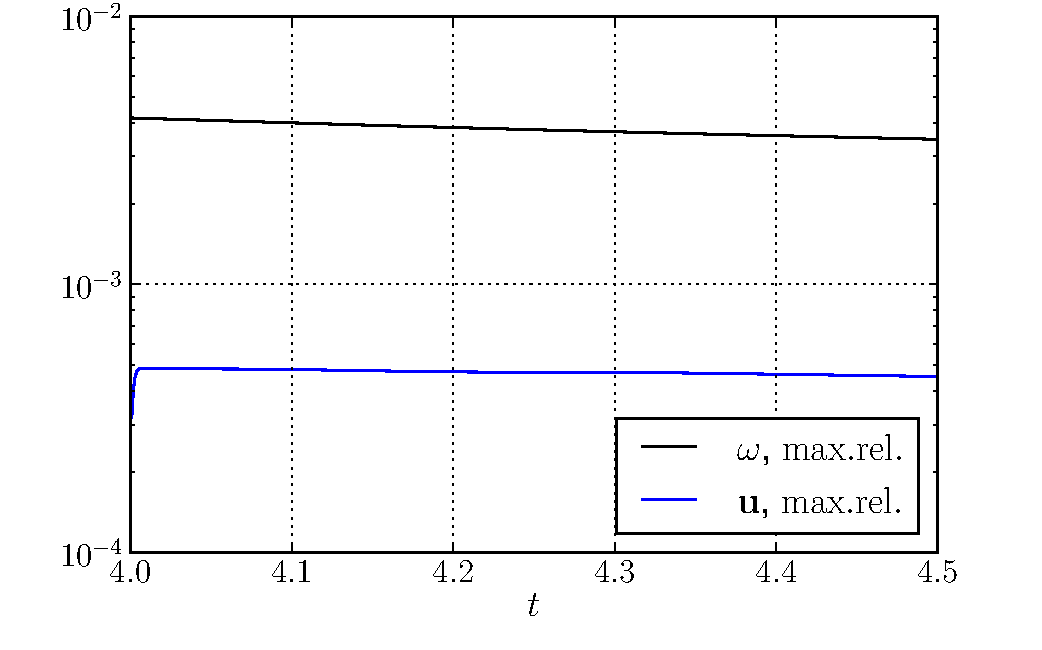
\includegraphics[width=0.7\linewidth]{./figures/eulerian/lambOseen_eulerian_wRelEvolution_compressed.pdf}
	\caption{Eulerian Lamb-Oseen relative vorticity evolution}
	\label{fig:lambOseen_eulerian_wRelEvolution}
	\end{figure}


	\begin{figure}[b]
        \centering
        \begin{subfigure}[b]{0.5\textwidth}
                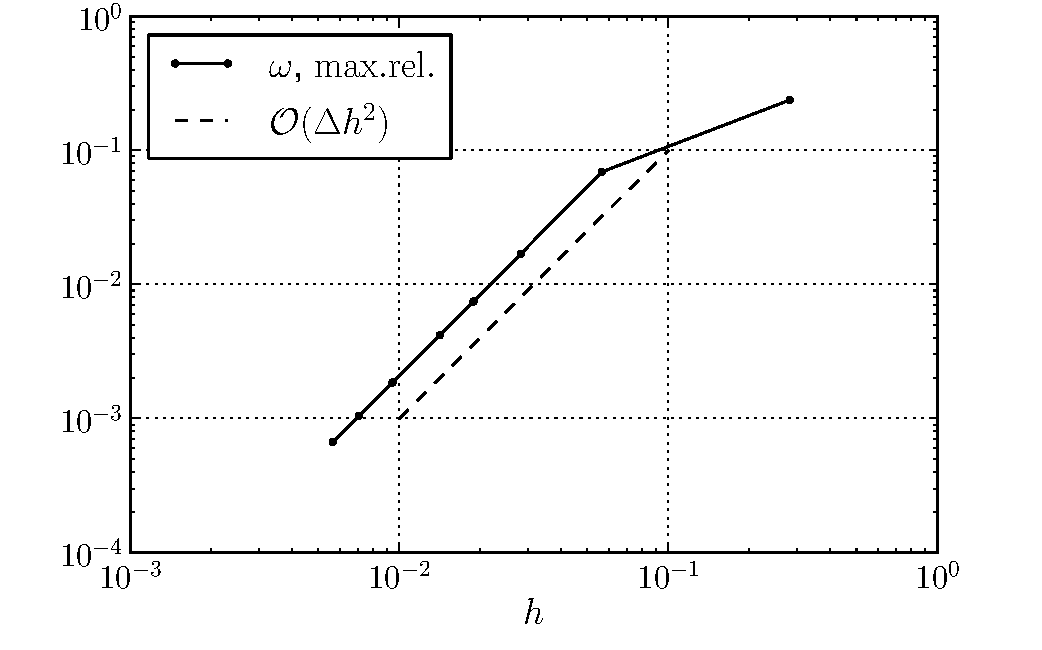
\includegraphics[width=\textwidth]{figures/eulerian/lambOseen_eulerianConvergence_dx_compressed.pdf}
                \caption{Lamb-Oseen dx convergence}
                \label{fig:lambOseen_eulerianConvergence_dx}
        \end{subfigure}%
        ~ %add desired spacing between images, e. g. ~, \quad, \qquad etc.
          %(or a blank line to force the subfigure onto a new line)
        \begin{subfigure}[b]{0.5\textwidth}
                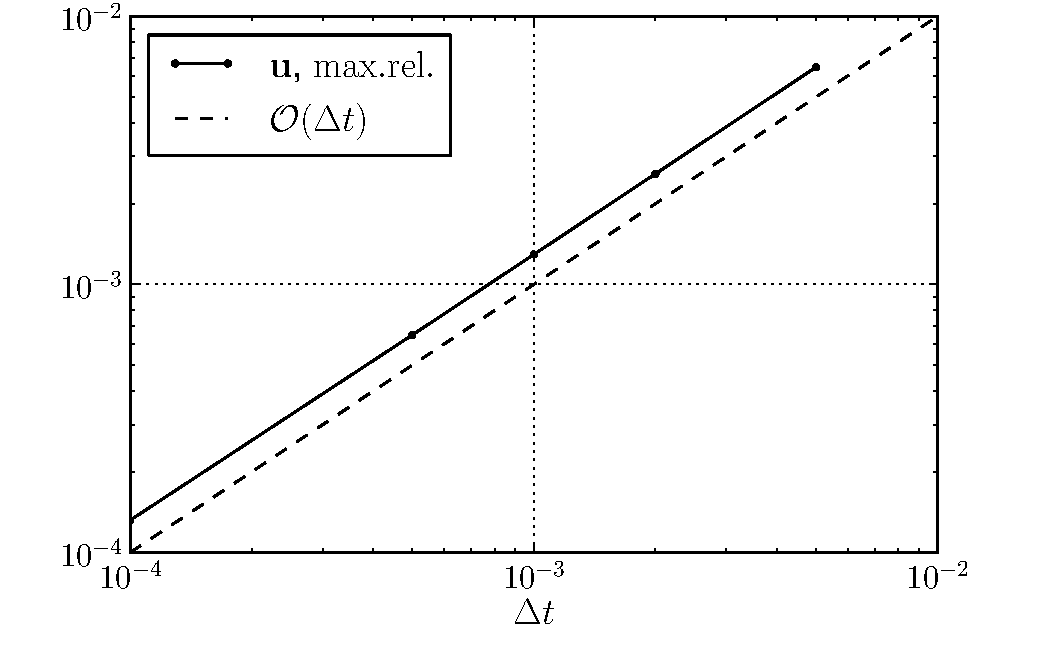
\includegraphics[width=\textwidth]{figures/eulerian/lambOseen_eulerianConvergence_dt_compressed.pdf}
                \caption{Lamb-Oseen dt convergence}
                \label{fig:lambOseen_eulerianConvergence_dt}
        \end{subfigure}
        \caption{Lamb-Oseen convergence}
        \label{fig:lambOseen_eulerianConvergence}
	\end{figure}	

\subsection{Clercx-Bruneau dipole collison at $Re=625$}

\subsection{Impulsively started cylinder at $Re=550$}

\section{Summary}

